\documentclass[a4paper,titlepage]{article}
\usepackage{frontespizio}
\usepackage[english]{babel}
\usepackage[utf8]{inputenc}
\usepackage{usecases}

\usepackage{tikz}
\usetikzlibrary{arrows,shadows} % for pgf-umlsd
\usepackage[underline=true,rounded corners=false]{pgf-umlsd}

\usepackage{enumitem}
\setitemize{noitemsep,topsep=0pt,parsep=0pt,partopsep=0pt}

\usepackage[a4paper, total={6in, 9in}]{geometry}



\begin{document}
\begin{frontespizio}
\Universita{Verona}
\Dipartimento{Informatica}
\Corso[Laurea]{Informatica}
\Titoletto{Software Engineering}
\Titolo{First project report}

\Candidato[VRGooby]{Giovanni Liboni}
\Candidato[VR359169]{Enrico Giordano}
\Candidato[VR359129]{Alberto Marini}
\Candidato[VR359333]{Alessandro Falda}

\Annoaccademico{2013-2014}
\end{frontespizio}


\newpage

\part{Introduction}

This report explain how a car parking system was implemented. The project was implemented in java language and the nodes of the system was converted into class, according to object oriented programming. 

~

Every entity was interpreted as a node of a grid that comunicate to another node with a channel; it use a particular node, Tx or Rx, wherewith send or receive a message. This remaind a particular design pattern called ''observer pattern``: it is a software design pattern in which an object, called the subject, maintains a list of its dependents, called observers, and notifies them automatically of any state changes, usually by calling one of their methods. It is mainly used to implement distributed event handling systems.

Every entity was a generalization of an abstract class called Node; infact an entity is a specialization of Node class.


\part{General pattern}

When a car arrive or exit to the park, the node ''car detector`` send a message to the node ''process unit``, that store the request (for future use) and send to the monitor the average number of car/hour and the number of free parking places. According to observer pattern, the subject (Sensor) notify the observer (Process Unit) that a new message is pending, so observer (Process Unit) receive istantly the message. After the computation, the Process Unit send in the same way the messages to the different displays.

So the sender node, when have to send a message, must call the receive method of the receiver node; in this way it was implemented an observer pattern.

    \begin{center}

    \centering
    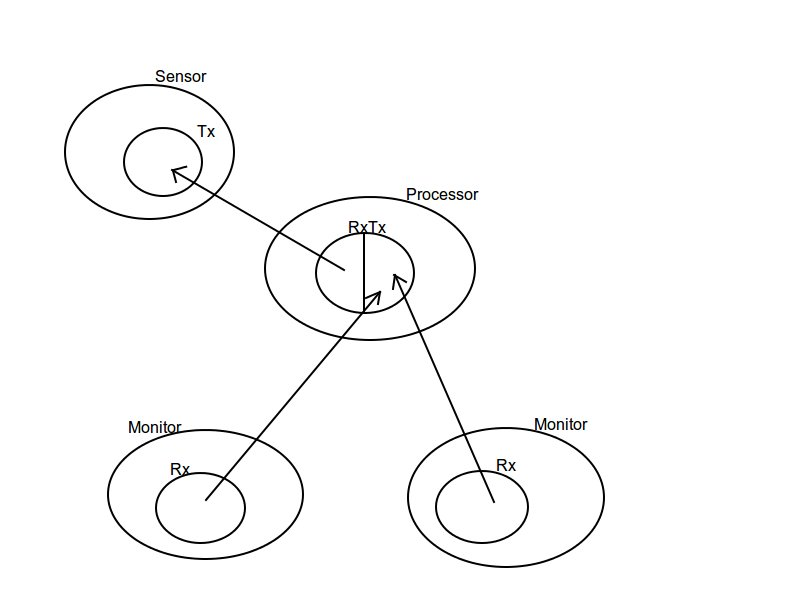
\includegraphics[scale=0.40]{pattern.jpg}

    \end{center}


There is a different type of node in this project, in particular:

\begin{itemize}[noitemsep,topsep=20pt,parsep=10pt,partopsep=20pt]

\item Detector: a sensor that controls car traffic (entering or exiting car); 
\item Processor: a processing unit that calculate average number of cars/hour anche number of free parking places;
\item Monitor: a display that shows the results of processing unit.

\end{itemize}

The comunication was implemented by ''Channel`` class, that create a link in a comunication grid. There are 2 tipes of Channel: WireChannel or WirelessChannel.

The Processor computation is done by a subnode called nodeComputation, that implement basic operation (sum, min, ecc...).

The comunication is done by a subnode called nodeCommunication, that implement:

\begin{itemize}[noitemsep,topsep=20pt,parsep=10pt,partopsep=20pt]

\item TxNode: must send a message (for Detector);

\item RxNode: must receive a message (for Monitor);

\item TxRxNode: must send and receive a message (for Processor);

\end{itemize}



\part{Simulation}

In the main class was created the detector, the processing unit and 3 monitor: a display for average number of car/hour, a display for number of free parking places and an additional display for car traffic.
The node is linked in the wireless grid and after that they can comunicate. A realtime clock in the processing unit simulate the time (for the average cars/hours) implemented with a thread. With the control button, the user can control the simulation.


\part{Questions}


\end{document}


